\documentclass[a4paper]{article}

\usepackage{INTERSPEECH2016}

\usepackage[hyphens]{url}
\usepackage{xcolor}
\usepackage{graphicx}
\usepackage{amssymb,amsmath,bm}
\usepackage{textcomp}
\usepackage{multirow}
\usepackage{multicol}
\usepackage{epstopdf}

\usepackage{listings}
\usepackage{color}

\definecolor{codegreen}{rgb}{0,0.6,0}
\definecolor{codegray}{rgb}{0.5,0.5,0.5}
\definecolor{codepurple}{rgb}{0.58,0,0.82}
\definecolor{backcolour}{rgb}{0.95,0.95,0.92}

\lstdefinestyle{mystyle}{
	backgroundcolor=\color{backcolour},   
	commentstyle=\color{codegreen},
	keywordstyle=\color{magenta},
	numberstyle=\tiny\color{codegray},
	stringstyle=\color{codepurple},
	basicstyle=\footnotesize,
	breakatwhitespace=false,         
	breaklines=true,                 
	captionpos=b,                    
	keepspaces=true,                 
	numbers=left,                    
	numbersep=5pt,                  
	showspaces=false,                
	showstringspaces=false,
	showtabs=false,                  
	tabsize=2
}

\lstset{style=mystyle}


\begin{document}

 % better line breaks
\ninept

\title{Laser Pointer Interactive System}

\makeatletter
\def\name#1{\gdef\@name{#1\\}}
\def\input@path{{C:/Users/Kan/Dropbox/LaserBoard/}}

\makeatother 
\name{\em Alex Taffe, Kan Kawabata, Vincent Velarde}
\address{School of Electrical, Computer and Energy Engineering}
	
\maketitle
\begin{abstract}
	In this paper we present a simple and low-cost method of creating an interactive laser pointer tracking sensing system using laser pointers, a webcam, projector and OpenCV library. This was done by, (1) applying a homography transformation on the camera's perspective to align the camera with the projector output, (2) separating the laser dots from background noise (3) extracting the coordinate of the laser dots from the thresholded image. 
	
	Given the above setup we were able to develop a few applications such as basic draw, controlling computer mouse, miniture games, etc. With three laser pointers we were also able to perform position tracking of the user through 3D resection.
	
\end{abstract}

\section{Introduction}
Technology such as smartboards, Nintendo's Wii, and Microsoft's Xbox Kinect use human motion and gestures to create an interactive experience for the user. The ability to fuse technologies with the environment is the first step for true virtual reality and augmented reality. Unfortunately these technologies can be expensive and complex, thus it puts a high skill and money barrier for people to buy and develop for such systems. This becomes a problem as it stagnates innovation and creativity in the industry and discourages potential developers. 
 
The motivation for this project is to create a motion sensing/tracking system with a laser pointer as an alternative to similar technologies that is currently on the market. Our system uses a laser pointer, laptop, webcam, and a projector all of which are either cheap or commonly available to the general public. Our software is based off of Python scripting language and OpenCV library both of which are open-source with great documentation, thus allowing anyone with basic programming skills to create and develop their own ideas. 

\section{Implementation}
In order to achieve our goals our system needs to be able to track multiple laser pointer dots and determine their position relative to the board. There are three stages to completing this task, a homography calibration stage to correct for camera perspective, a stage to threshold camera feed to filter out noise and varied light intensities and detect laser dot, and finally contour detection stage for calculating multiple laser dot positions. Figure \ref{fig:3stage} shows the initial input and output of the first two stages. Once these steps are completed the binary image will then be used to calculate the coordinates of the laser pointer position using find contour and centroid formula. 

\begin{figure}
	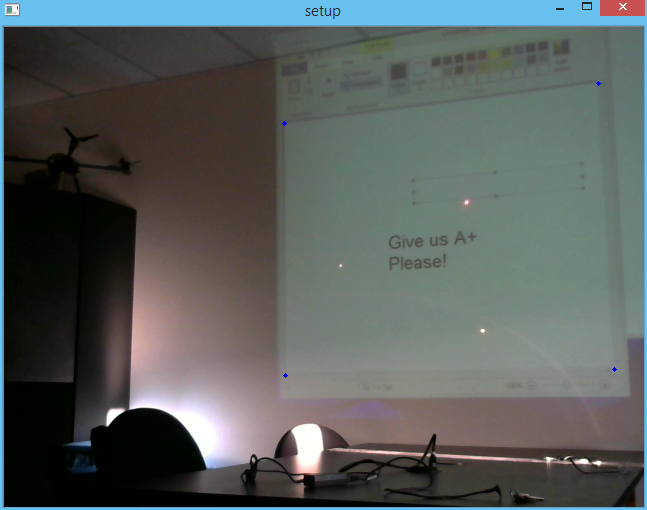
\includegraphics[width=\linewidth]{raw_feed.png} \newline
	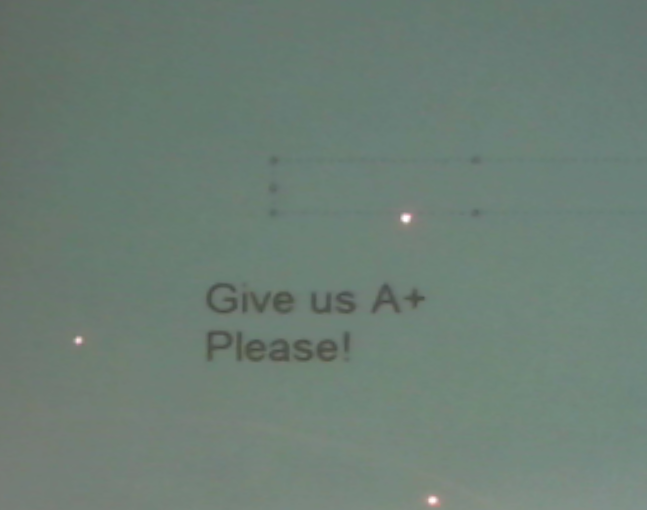
\includegraphics[width=\linewidth]{transformed.png} \newline
	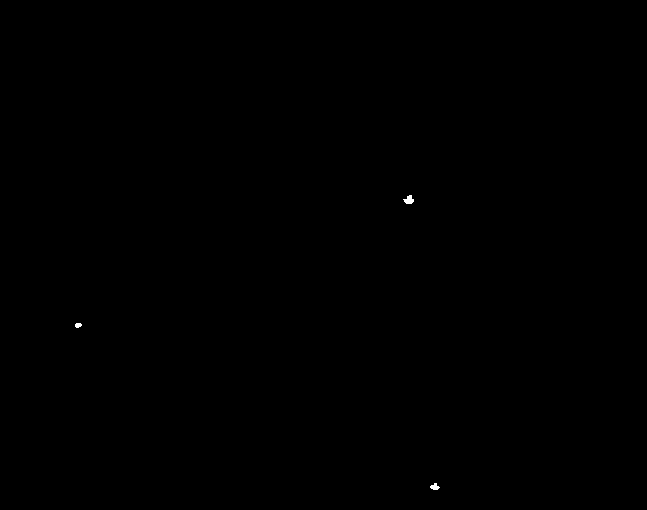
\includegraphics[width=\linewidth]{bwimage.png}
	\caption{(Top)raw camera feed (middle)perspective transformed (bottom)intensity thresholded}
	\label{fig:3stage}
\end{figure}

\subsection{Homograph transformation}
The camera calibration was done using a OpenCV's perspective transform function. The Idea is to determine the homography matrix that transforms the camera's perspective of the environment to the head on view of the board. 

\begin{equation}
\begin{bmatrix}
x' \\ y' \\ z'\\ w'
\end{bmatrix} = H * \begin{bmatrix}
 x \\ y \\ z \\ 1
\end{bmatrix}
\end{equation}

In class we shown how to do this using the 8 point algorithm \cite{hartley1997defense} however because the camera captures the projection on the wall (which is co-planer) this transformation can be thought of as a simple 2D mapping problem. 

\subsection{Robust noise filtering}
One of the challenges to the project is finding a robust way of filtering out noise and varied lighting while still detecting the laser dot. Initially we set a global threshold intensity where any pixel with intensity greater than some value would be considered as a laser dot and anything below as background. However this required the user to personally adjust the global thresholding manually as the program has no way of knowing the optimal threshold. Additionally this method is not robust to difference in lighting, a brighter lit area would be more sensitive to noise while a darker area would not detect the laser dots. 

To solve this issue, during calibration the camera will capture a couple seconds of background image with no laser dot present, then it will select for each pixel the maximum intensity detected for the duration and use that as a basis for thresholding. This method accounts for difference in lighting as each pixel has their own thresholding value associated with it and it is also automatically done by the system.

\subsection{Find Contour and coordinate Estimation}
The thresholding produces a black and white image of the detected laser dots. We want to convert this image to a list of coordinates of where the dots are located. To do this we use OpenCV's findContours which takes in an eight bit single channel image and performs the algorithm in \cite{suzuki1985topological} and returns a vectors of points that each correspond to a particular laser dot in the camera feed. 

Two algorithms are described in \cite{suzuki1985topological}, one that starts a border following algorithm on borders, once a start condition is fulfilled. The borders are followed in the order they are encountered during a raster scan. Algorithm number two is a modified version of the first, that searches exclusively for outer borders. 

Algorithm one starts with a line by line scan of the image from left to right, until the start condition is satisfied. \cite{suzuki1985topological} defines a coordinate system where i represents rows and j represents columns with rows (i) increase from top to bottom and columns(j) increase from left to right. The start condition is defined as when and one is encountered during the scan. The border is then classified as either an outer border or a hole border. If a one preceded by a zero then the border is classified as a outer border, otherwise if the one is succeeded by a zero then it is a hole border. Holes are defined as sections of 8- connected zero pixels, whereas the opposite 1-components are classified as 4-connected 1 pixels. If a one is preceded and succeeded by a zero it is classified as an outer border. Each pixels in the current border is then assigned a unique number then the bordered is followed until it ends. If the current pixels is (i,j) then if (i,j + 1) is a zero the pixel is assigned a negative number otherwise it is assigned a positive number. Border following occurs according to the classical method in \cite{rosenfeld2014digital} then the algorithm returns to the start point of the border and continues the raster scan. The parent border of the current border is also recorded and classified as an outer border or a hole border according to the Table 1 in \cite{suzuki1985topological}. 

\begin{figure}
	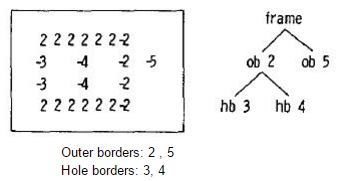
\includegraphics{contour.png}
	\caption{Example contoured binary image \cite{suzuki1985topological}}
\end{figure}

Algorithm two is the same as algorithm one except hole borders are not recorded only the outermost borders of a section of connected components. The OpenCV library contains other options for detecting blobs in an image the findContours algorithm is low cost in terms of processing power compared to functions in the library like houghCircles for example and performed successfully during the implementation of our project. 

Once the coordinates are determined we can then find the centroid using the centroid formula,
\begin{equation}
\bar{x} = \frac{\sum\limits_{x = x_{min}}^{x_{max}}{x P_x(x)}}{\sum\limits_{x = x_{min}}^{x_{max}}{P_x(x)}}, \quad
\bar{y} = \frac{\sum\limits_{y = y_{min}}^{y_{max}}{y P_y(y)}}{\sum\limits_{y = y_{min}}^{y_{max}}{P_y(y)}}
\end{equation}

Where $P_x(x)$ and $P_y(y)$ are the sum of pixels in that column or row where laser dot is detected. 

\section{Applications and Tech Demos}
Once the system can track laser dots and find their coordinates, the applications are mostly determined by the developer's own creativity and imagination. 

For this project we created a variety of tech demos (see youtube playlist \cite{techDemos} and code) that shows the possible application this system can have. These include:

\begin{itemize}
	\item Basic Draw Function - ability to draw on canvas (see figure \ref{fig:hello})
	\item Mouse Function - ability to move and click computer mouse with laser dot
	\item Maze Demo - game to move through a maze without hitting walls
	\item Target Shooting Demo - game to shoot at targets displayed
	\item Pong game - control the paddles with laser dots (see figure \ref{fig:pong})
	\item Position Tracking Demo - see next section

\end{itemize}

\begin{figure}
	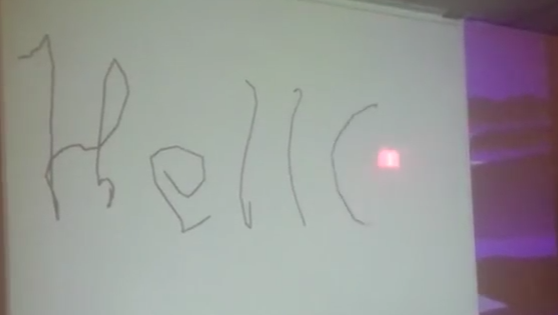
\includegraphics[width=\linewidth]{hello.png}
	\caption{screen shot of basic draw}
	\label{fig:hello}
\end{figure}

\begin{figure}
	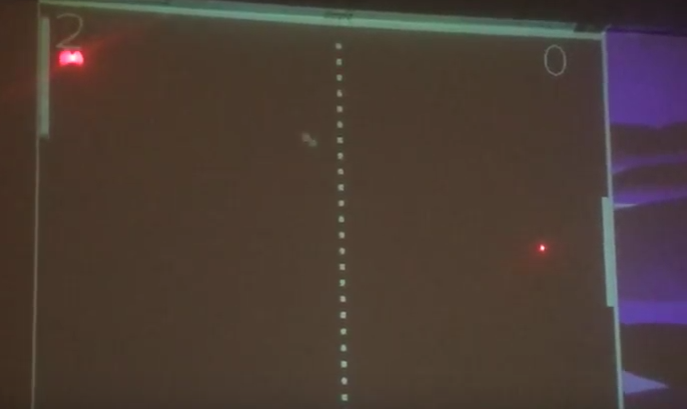
\includegraphics[width=\linewidth]{pong.png}
	\caption{screen shot of pong game}
	\label{fig:pong}
\end{figure}

\section{Position Estimation with 3D Re-sectioning}
An unconstrained object in 3D motion has six degrees of freedom: three translational and three rotational.  Given the projections of three lines on a canvas all which intersect a common source, is it possible to find the position of the source? In finding the solution to this problem, it was uncovered that a similar problem, called the Three-Dimension Resection Problem (3DR) had been solved well in literature. The 3DR problem is to determine the lengths of a tetrahedral given three angles between the sides and the lengths opposite of the angles. The solution, though well documented, is not trivial and with multiple solutions. It is common instead to try to numerically solve the proper solution. Our problem, that of finding the position of the source of three lasers given their intersection with a plane, is somewhat more involved than just solving the 3DR problem.  What follows is a breakdown of the procedure including approaches to deal with practical issues that arise.

\subsection{Solving for the Lengths}
If we examine the geometry that the three lasers make with the canvas, the shape that forms is an irregular tetrahedral. If we consider what we know, the end points of the lasers and the angles between the lasers, the problem of solving for the lengths of the lasers is exactly solving the 3DR problem. Fortunately, the geometry is rather straight forward as the problem boils down to solving the three equations defined by the law of cosines. The issue is this problem has no explicit solution that is trivial, and those explicit solutions which exist, they do not guarantee unique solutions. Here we opt to solve this problem numerically. 
\begin{figure}
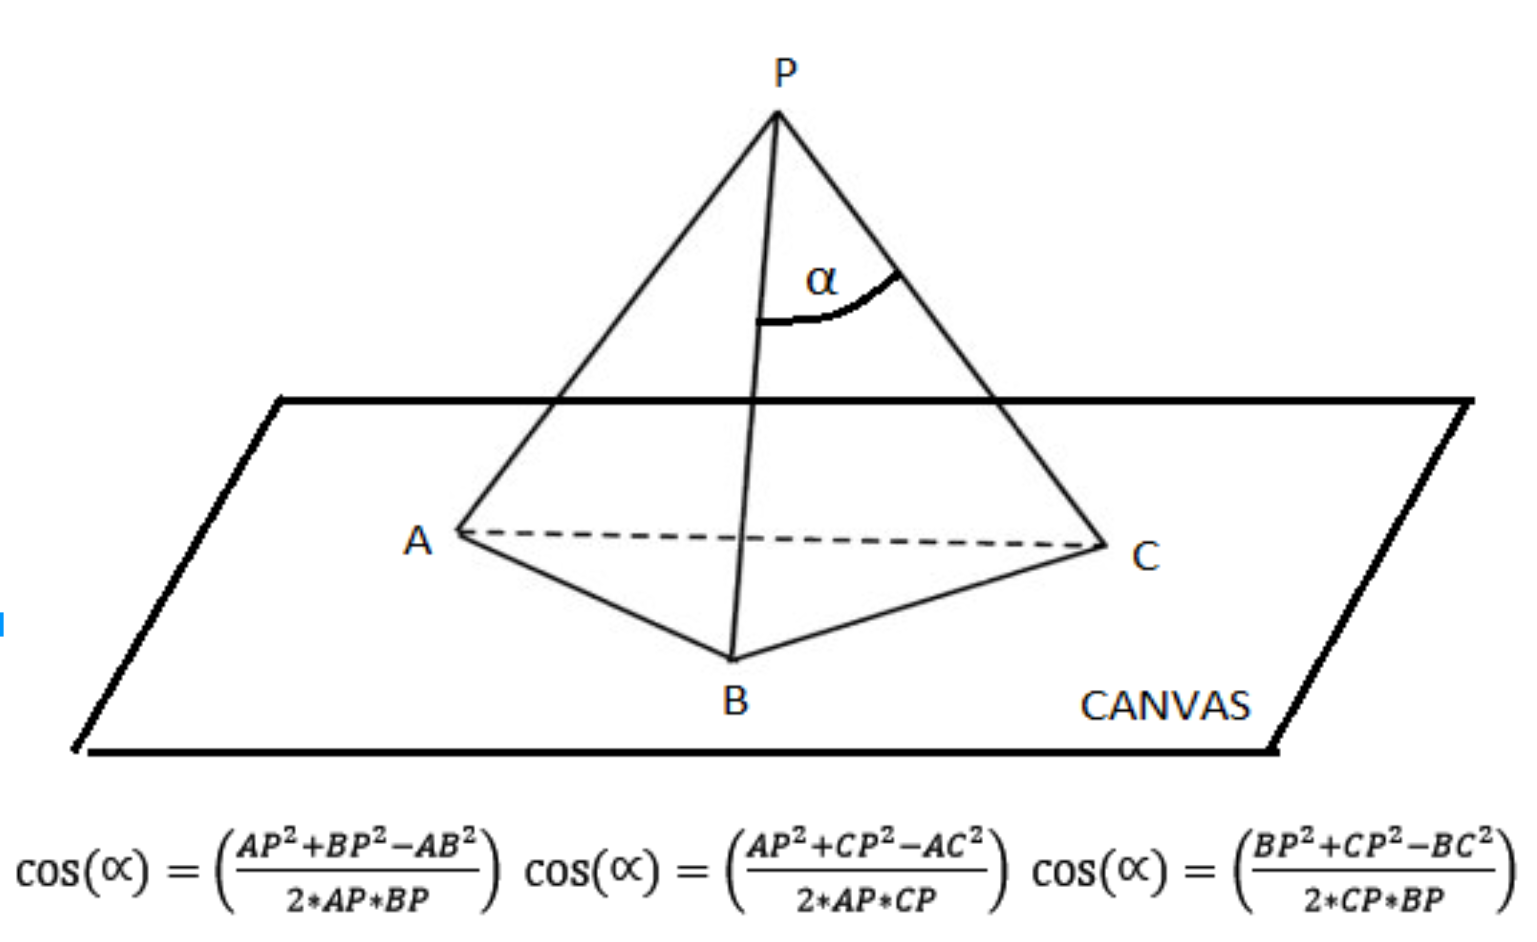
\includegraphics[width=7cm]{resection_fig.png}
\caption{Geometry of resection problem}
\end{figure}

\subsection{Solving for the Direction Vectors}
To obtain the source coordinates, we are not just satisfied knowing the lengths of the lasers, but also their directions. With this knowledge we can directly calculate the source position. To solve for the direction vectors knowing the lengths of the lasers, the end points of the lasers, and finally knowing that the lasers have a common source, we can set up three equations vector equations defined by the equation of a line, restricting the lines to pass through one of the three lasers end points A,B,C as well as the common source P. 

\begin{figure}
	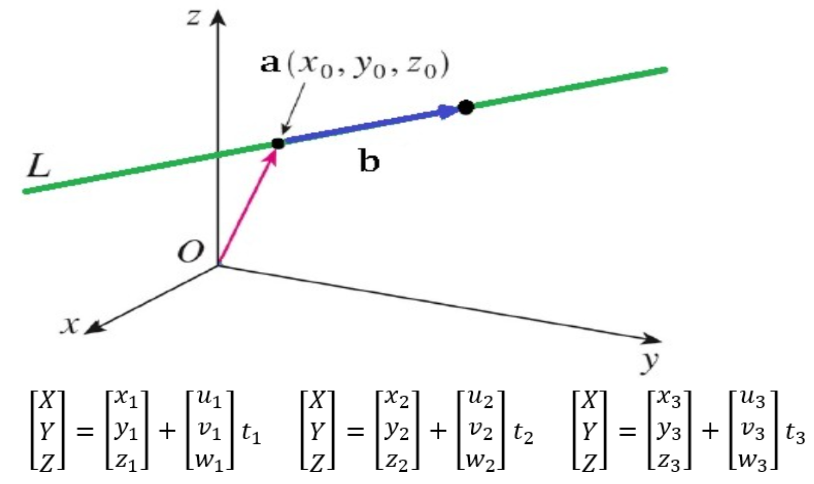
\includegraphics[width=7cm]{resection_fig2.png}
	\caption{Parametric Equation of Line in 3D}
\end{figure}

What we obtain are nine algebraic equations with 9 unknowns corresponding to the three entries of the three direction vectors we are interested in. Here $t_1$,$t_2$,$t_3$ represent the lengths of the lasers found, $x_n$,$y_n$,$z_n$ the coordinates of the laser points on the canvas, and finally $u_n$,$v_n$,$w_n$ the unit direction vectors each laser. 

\begin{equation}
\resizebox{\linewidth}{!}{$
\begin{bmatrix}
x_2 - x_1 \\
y_2 - y_1 \\
z_2 - z_1 \\
x_3 - x_1 \\
y_3 - y_1 \\
z_3 - z_1 \\
x_2 - x_3 \\
y_2 - y_3 \\
z_2 - z_3 
\end{bmatrix} = 
\begin{bmatrix}
t_1 & 0   & 0   &-t_2 & 0   & 0   & 0   & 0   & 0   \\
0   & t_1 & 0   & 0   &-t_2 & 0   & 0   & 0   & 0   \\
0   & 0   & t_1 & 0   & 0   &-t_2 & 0   & 0   & 0   \\
t_1 & 0   & 0   & 0   & 0   & 0   &-t_3 & 0   & 0   \\
0   & t_1 & 0   & 0   & 0   & 0   & 0   &-t_3 & 0   \\
0   & 0   & t_1 & 0   & 0   & 0   & 0   & 0   &-t_3 \\
0   & 0   & 0   &-t_2 & 0   & 0   & t_3 & 0   & 0   \\
0   & 0   & 0   & 0   &-t_2 & 0   & 0   & t_3 & 0   \\
0   & 0   & 0   & 0   & 0   &-t_2 & 0   & 0   & t_3 
\end{bmatrix}
\begin{bmatrix}
u_1\\
v_1\\
w_1\\
u_2\\
v_2\\
w_2\\
u_3\\
v_3\\
w_3
\end{bmatrix} $}
\end{equation}

\begin{equation}
\resizebox{\linewidth}{!}{$
\begin{bmatrix}
x_2 - x_1 \\
y_2 - y_1 \\
z_2 - z_1 \\
x_3 - x_1 \\
y_3 - y_1 \\
z_3 - z_1 \\
x_2 - x_3 \\
y_2 - y_3 \\
z_2 - z_3 
\end{bmatrix} = 
\begin{bmatrix}
t_1 & 0   & 0   &-t_2 & 0   & 0   & 0   & 0   & 0   \\
0   & t_1 & 0   & 0   &-t_2 & 0   & 0   & 0   & 0   \\
0   & 0   & t_1 & 0   & 0   &-t_2 & 0   & 0   & 0   \\
t_1 & 0   & 0   & 0   & 0   & 0   &-t_3 & 0   & 0   \\
0   & t_1 & 0   & 0   & 0   & 0   & 0   &-t_3 & 0   \\
0   & 0   & t_1 & 0   & 0   & 0   & 0   & 0   &-t_3 \\
0   & 0   & 0   &-t_2 & 0   & 0   & t_3 & 0   & 0   \\
0   & 0   & 0   & 0   &-t_2 & 0   & 0   & t_3 & 0   \\
0   & 0   & 0   & 0   & 0   &-t_2 & 0   & 0   & t_3 
\end{bmatrix}
\begin{bmatrix}
X_1/||V_1||\\
Y_1/||V_1||\\
Z_1/||V_1||\\
X_2/||V_2||\\
Y_2/||V_2||\\
Z_2/||V_2||\\
X_3/||V_3||\\
Y_3/||V_3||\\
Z_3/||V_3||
\end{bmatrix} $}
\end{equation}

At first glance these equations look linear, and they are, however we must restrict the vectors found to be unit vectors, scaled by the previous found lengths. We place this restraint by dividing each vector by its norm. In doing so the system becomes nonlinear, and again a rather nasty set of equations to solve for. How do we then solve for the unit direction entries? Our solution is to solve them numerically.

\begin{equation}
\begin{aligned}
V_1=[X_1 \ Y_1 \ Z_1 ], & V_2=[X_2 \ Y_2 \ Z_2 ], & V_3=[X_3 \ Y_3 \ Z_3 ] \\
D_a=\frac{V_1}{\|\|V_1\|\|}, & D_b=\frac{V_2}{\|\|V_2\|\|}, & D_c=\frac{V_3}{\|\|V_3\|\|}
\end{aligned}
\end{equation}

\subsection{Solving for Position}
Now that we have obtained the lengths and direction vectors of the lasers and that we know the coordinates of the laser end points A,B,C we can now obtain the source position simply by vector subtraction. 

\begin{figure}
	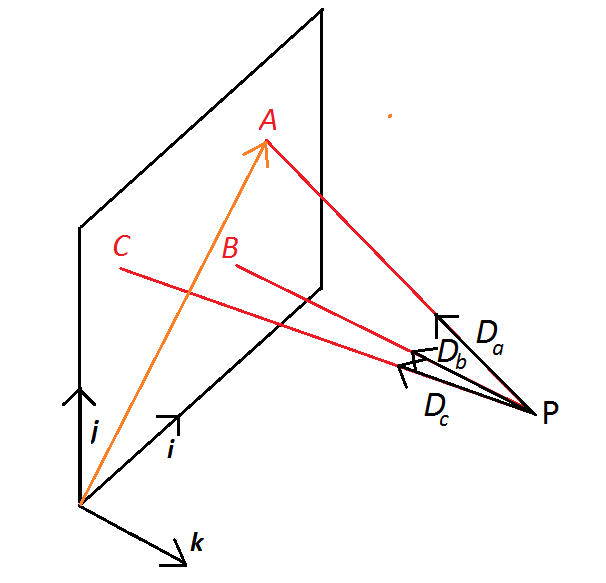
\includegraphics[width=7cm]{resection_fig3.png}
	\caption{Directional vector and length visualization}
\end{figure}

\begin{equation}
P_{avg}=\frac{(A-D_a t_1 )+ (B-D_b t_2 )+(C-D_c t_3 )}{3}
\end{equation}

\subsection{Solving for Orientation (Roll,Pitch,Yaw)}
If we consider an arbitrary rotation matrix, there are 9 unknowns. These entries are determined by the angles, axis, and order of the consecutive rotations in sequence. For roll, pitch , yaw the order is a 3-2-1 rotation starting with yaw, pitch, then roll. The rotation matrix has the following form:
\begin{equation}
\resizebox{\linewidth}{!}{$
R(\phi,\theta,\psi) = \begin{bmatrix}
c \psi c \theta & c \psi s \phi s \theta - c s \psi & s \phi s \psi + c \phi c \psi s \theta \\
c \theta s \psi & c \phi c\ psi + s s & c \phi s \psi s \theta - c \psi s \phi \\ 
-s \theta & c \theta s \phi & c \phi c \theta)
\end{bmatrix} = \begin{bmatrix}
r_{11} & r_{12} & r_{13}\\
r_{21} & r_{22} & r_{23}\\
r_{31} & r_{32} & r_{33}
\end{bmatrix} $}
\end{equation}
\begin{equation}
\begin{aligned}
\phi=&\tan^{-1}(r_{21}/r_{11} ) &\\
\theta_1=&\tan^{-1}(-r_{31}/\sqrt(r_{32}^2+r_{33}^2 )), & \quad \theta \in(-\pi/2,\pi/2) \\
\theta_2=&\tan^{-1}(-r_{31}/\sqrt(r_{32}^2+r_{33}^2 )), & \quad \theta \in (\pi/2,3\pi/2) \\
\psi=&\tan^{-1}(r_{32}/r_{33} ) &
\end{aligned}
\end{equation}

Yaw, pitch, and roll angles can be solved by examining elements. It is desirable to define angles in terms of tan2, which keeps track of the quadrant. There are two different solutions for pitch given the expected quadrant it should be in. For our application, we expect pitch to be between -pi/2 and pi/2.


Next, we need to determine how to find the rotation matrix for each update. This is done by considering an initial orientation with the initial direction vectors of the lasers $VA_o$,$VB_o$,$VC_o$ and the current direction vectors of the lasers VA,VB,VC to determine the rotation matrix R which acts to map the two.
\begin{equation}
\begin{bmatrix}
	r_{11} & r_{12} & r_{13}\\
	r_{21} & r_{22} & r_{23}\\
	r_{31} & r_{32} & r_{33}
\end{bmatrix} \begin{bmatrix}
DA_{xo} \\ DA_{yo} \\ DA_{zo}  
\end{bmatrix} = \begin{bmatrix}
DA_{x} \\ DA_{y} \\ DA_{z}  
\end{bmatrix}
\end{equation} 
\begin{equation}
\begin{bmatrix}
r_{11} & r_{12} & r_{13}\\
r_{21} & r_{22} & r_{23}\\
r_{31} & r_{32} & r_{33}
\end{bmatrix} \begin{bmatrix}
DB_{xo} \\ DB_{yo} \\ DB_{zo}  
\end{bmatrix} = \begin{bmatrix}
DB_{x} \\ DB_{y} \\ DB_{z}  
\end{bmatrix}
\end{equation}
\begin{equation}
\begin{bmatrix}
r_{11} & r_{12} & r_{13}\\
r_{21} & r_{22} & r_{23}\\
r_{31} & r_{32} & r_{33}
\end{bmatrix} \begin{bmatrix}
DC_{xo} \\ DC_{yo} \\ DC_{zo}  
\end{bmatrix} = \begin{bmatrix}
DC_{x} \\ DC_{y} \\ DC_{z}  
\end{bmatrix}
\end{equation}

Here we have 9 equations in 9 unknowns, as such we can solve this linear system. Here, because of error introduced into the system, we opt to find the nearest solution, in case one does not exist. The system can be rewritten to solve for the components of R.
\begin{equation}
\resizebox{\linewidth}{!}{$
\begin{bmatrix}
DA_x \\DA_y \\DA_z \\DB_x \\DB_y \\DB_z \\DC_x \\DC_y \\DC_z 
\end{bmatrix}_b = 
\begin{bmatrix}
DA_{xo} & 0      & 0      & DA_{yo}& 0      & 0      & DA_{zo}& 0      & 0      \\
0       & DA_{xo}& 0      & 0      & DA_{yo}& 0      & 0      & DA_{zo}& 0      \\
0       & 0      & DA_{xo}& 0      & 0      & DA_{yo}& 0      & 0      & DA_{zo}\\
DB_{xo} & 0      & 0      & DB_{yo}& 0      & 0      & DB_{zo}& 0      & 0      \\
0       & DB_{xo}& 0      & 0      & DB_{yo}& 0      & 0      & DB_{zo}& 0      \\
0       & 0      & DB_{xo}& 0      & 0      & DB_{yo}& 0      & 0      & DB_{zo}\\
DC_{xo} & 0      & 0      & DC_{yo}& 0      & 0      & DC_{zo}& 0      & 0      \\
0       & DC_{xo}& 0      & 0      & DC_{yo}& 0      & 0      & DC_{zo}& 0      \\
0       & 0      & DC_{xo}& 0      & 0      & DC_{yo}& 0      & 0      & DC_{zo}
\end{bmatrix}_A
\begin{bmatrix}
r_{11}\\ r_{21}\\ r_{31}\\ 
r_{12}\\ r_{22}\\ r_{23}\\
r_{13}\\ r_{23}\\ r_{33}
\end{bmatrix}_x $}
\end{equation}
The above equation can then be solved using the least squares formula,
\begin{equation}
x = (A^T A)^{-1} A^T b
\end{equation}

\subsection{Methods of Implementation}
MATLAB and Python’s fsolve
In solving the lengths and directions we applied a numeric solver which requires an initial value to process. Unfortunately providing just any initial value will not guarantee the correct value. There are two simple approaches which attempt to avoid the wrong solution. The first approach is to simply use the previous solutions for lengths and directions. This works assuming that the both translation and rotation are slow. 
Approach 1:

\begin{equation}
Lo_i = L_{i-1}, \qquad Vo_i = V_{i-1}
\end{equation}


While it may be reasonable to limit the translation, limiting the rotation is simply not realistic. It may be difficult for one to translate a great distance between updates, but it is very feasible to change orientation with the flick of a wrist. For this operation we instead use the previous position estimate and the new known laser end points to estimate the direction and length of the lasers.

Approach 2:   

\begin{figure}
	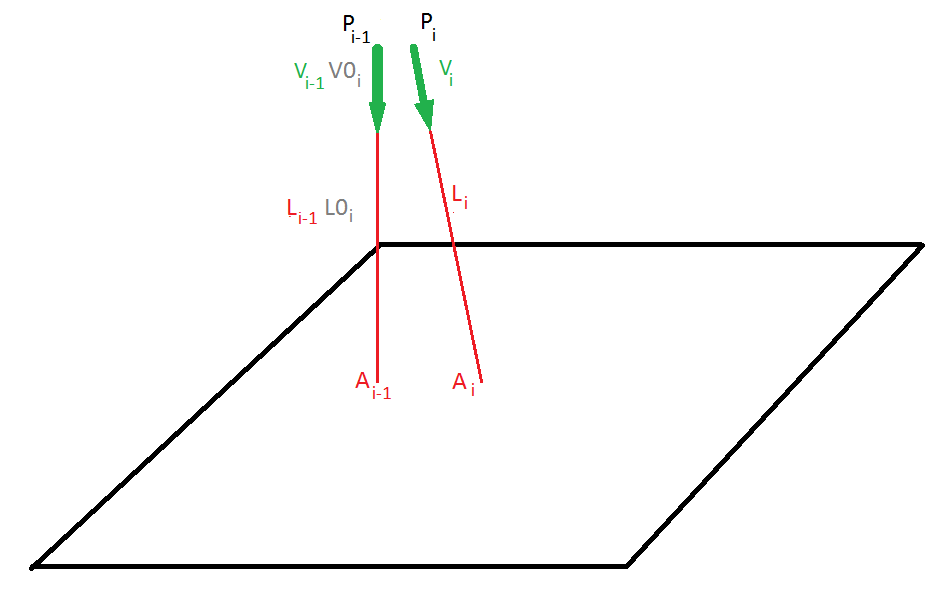
\includegraphics[width=\linewidth]{resection_fig4.png}
	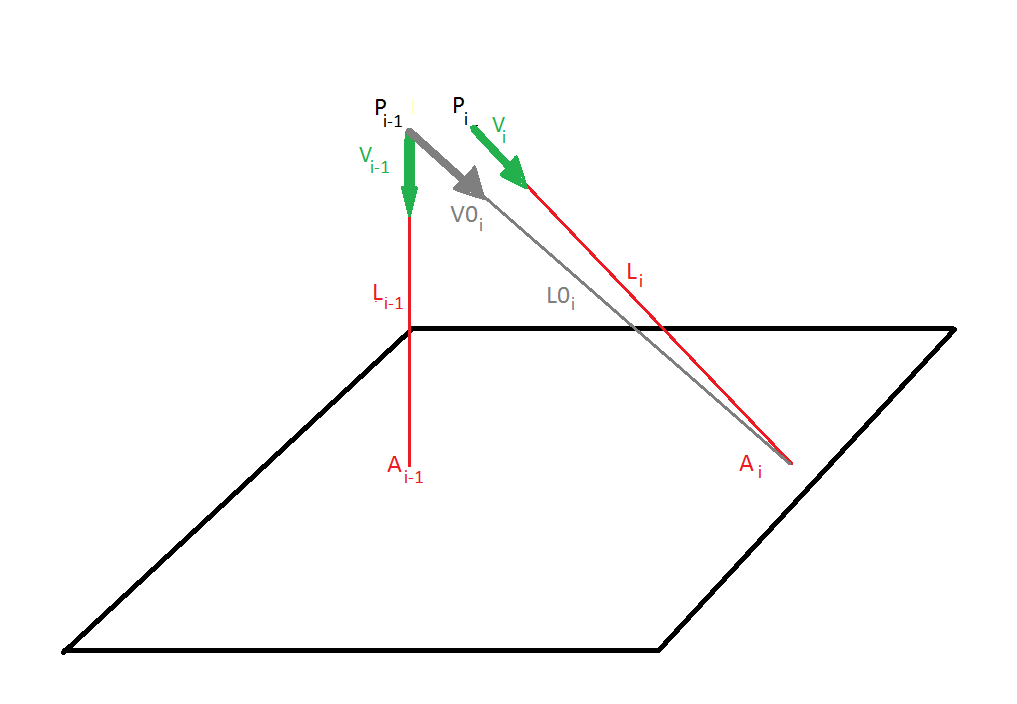
\includegraphics[width=\linewidth]{resection_fig5.png}
	\caption{Approach 1 visualization (above) approach 2 visualization (below)}
\end{figure}

\begin{equation}
	Lo_i = L_{i-1}, \qquad Vo_i = \frac{A_i - P_{i-1}}{||A_i -P_{i-1}||}
\end{equation}

Simulations of both cases within MATLAB and Python show that the second approach is more robust to fast orientations changes which are more likely to occur than quick displacements. Both the lengths of the lasers and their direction vectors were solved using MATLAB’s and Pythons fsolve(). Computation time using MATLAB was on the order of .1 seconds compared to Pythons .001 seconds. 

\subsection{Initialization}
Both solving the lengths and directions of the lasers use a numeric solver which requires the prior position for guessing an initial value. Also the angles between each of the lasers are required. To obtain roll, pitch, and yaw, the initial direction vectors of the lasers are required. All of these values can be found during an initialization procedure upon start up. 
Initial Position:
Here we need to know a good guess for position in order to estimate the lengths and directions of the lasers as mentioned earlier. Here we opt to simply ask the user to stand at the left-lower hand corner of the screen corresponding to the origin, and then stand an equal distance from the board compared to the height of the board. For example, if the board is 2m tall, the user would stand 2m away from the lower left hand corner. Because this position is known, this is used to initialize position.
\begin{equation}
P_o = \begin{bmatrix}
0\\ 0 \\-2
\end{bmatrix} \text{(meters)}
\end{equation}

\subsection{Initial angles}
In order to obtain estimates of our orientation, we must compare the unit direction vectors of the three lasers at a given point in time to an initial, zeroed angle, orientation. There are two ways to do this. The first way is to simply predefine an zero orientation and a corresponding set of laser directions. This is only feasible if you know the angles between the lasers. For example lets assume laser A is pointing in the negative  K-axis, laser B is made by rotating laser A by an angle AB about the J-axis, and laser C is defined by the restrictions on angle AC and BC. 
The difficulty is in calculating the direction of laser C, because the axis of rotation is not known trivially. The system is constrained, so a relation can be found, however for the purpose of this project, we opted to use the initial direction vectors to define the zeroed angles. This is done by using the initial position and the measured end laser points, and back solving the direction vectors.

\begin{equation}
\begin{bmatrix}
L_{Ao}\\ L_{Bo} \\ L_{Co}
\end{bmatrix} = \begin{bmatrix}
||A_o - P_o|| \\ ||B_o - P_o|| \\||C_o - P_o|| 
\end{bmatrix}
\end{equation}

\begin{equation}
D_{Ao} = \frac{A_o-P_o}{L_Ao}, \quad D_{Bo} = \frac{B_o-P_o}{L_Bo}, \quad D_{Co} = \frac{C_o-P_o}{L_Co}
\end{equation}

\subsection{Defining angles between lasers}
So far we have assumed that we know the angles between the lasers, however if the lasers are not mounted precision, the angles may not be known well. In our case the mounting hardware for the lasers were not rigid as to allow for movement of the lasers to ensure that they intersected a point in space. So every time we tested, the lasers angles may have changed. To get around this issue, we simply back calculated the angles assuming that the initial position was known, as described above.  

\begin{equation}
\begin{bmatrix}
\alpha_{AB}\\ \alpha_{AC} \\ \alpha_{BC}
\end{bmatrix} = \begin{bmatrix} \cos^{-1}(\frac{AP^2+BP^2-AB^2}{2AP*BP}) \\ \cos^{-1}(\frac{AP^2+CP^2-AC^2}{2AP*CP}) \\ \cos^{-1}(\frac{BP^2+CP^2-BC^2}{2BP*CP})
\end{bmatrix}, \quad
\begin{bmatrix} AP\\BP\\CP
\end{bmatrix} = \begin{bmatrix} LA_o\\LB_o\\LC_o
\end{bmatrix}
\end{equation}

In the likely case that the angles found are note equal, the program must be able to track which laser points belong to which laser. In our application we used OpenCV’s contour function, which separates blobs, however it does not keep track of which blobs are which, but instead applies a kernel from the top left to bottom right. The implication of this is that the lasers eventually swap order and the position estimation fails. 
A simple solution to resolve this is to assume that given a correct set of prior laser points tags, that the correct tags for the next iteration will result minimizing the displacements. This was found to resolve the swapping issue. 
\begin{equation}
\begin{bmatrix}
A_i \\ B_i \\ C_i
\end{bmatrix} =  \begin{bmatrix}
P_j\\
P_k\\
P_l
\end{bmatrix}
\end{equation}
where j, k, l satisfy,
\begin{equation}
\underset{j,k,l}{\operatorname{argmin}} (||A_{i-1} -P_j|| + ||B_{i-1} -P_k|| + ||C_{i-1} -P_l||) 
\end{equation}
for j,k,l = 1,2,3 and $j \neq k \neq l$.

\subsection{Simulation}
Two different simulations were carried out, one in MATLAB to visualize the results, and one ported to Python which was the platform used for the project. The MATLAB simulation proved to be a very valuable tool in evaluating the validity of the numeric solutions, though computation time proved to be slow on the order of a tenth of a second. Here it was discovered that using the prior position plus the new laser positions to estimate the new laser lengths and directions \ref{fig:long2} proved to be better than just using the past directions and lengths \ref{fig:long1}. 

\begin{figure*}
	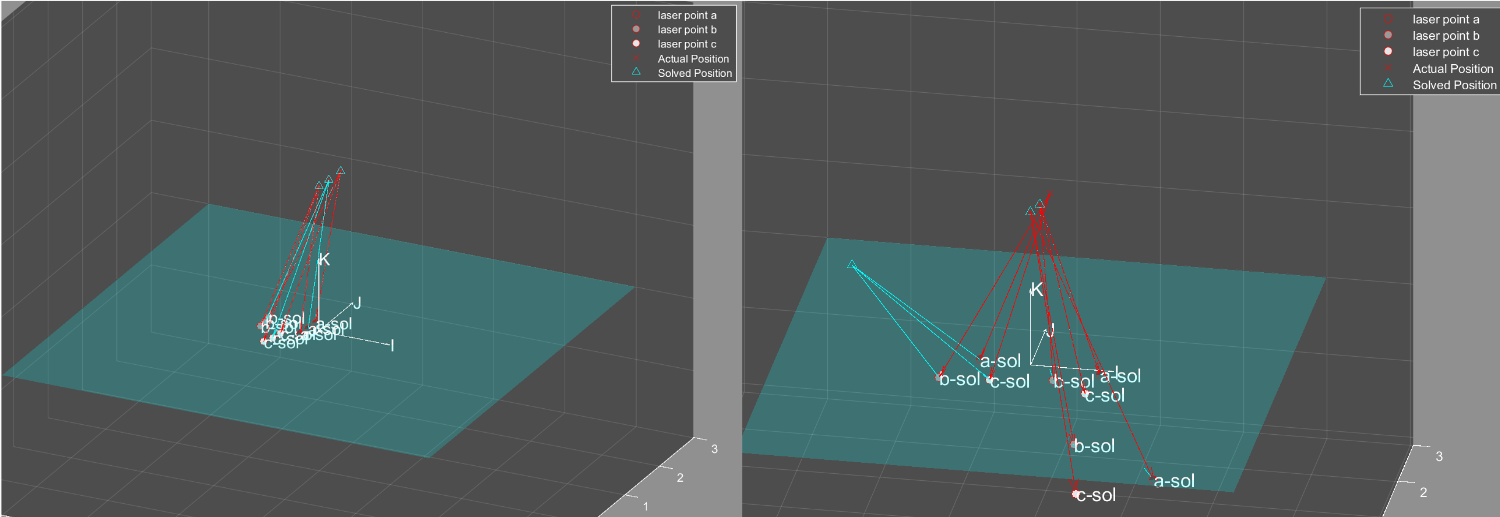
\includegraphics[width=\textwidth]{resection_fig6}
	\caption{Estimation based on prior lengths and direction vectors  small changes in orientation(Left) large changes in orientation (Right) }
	\label{fig:long1}
\end{figure*}


\begin{figure*}
	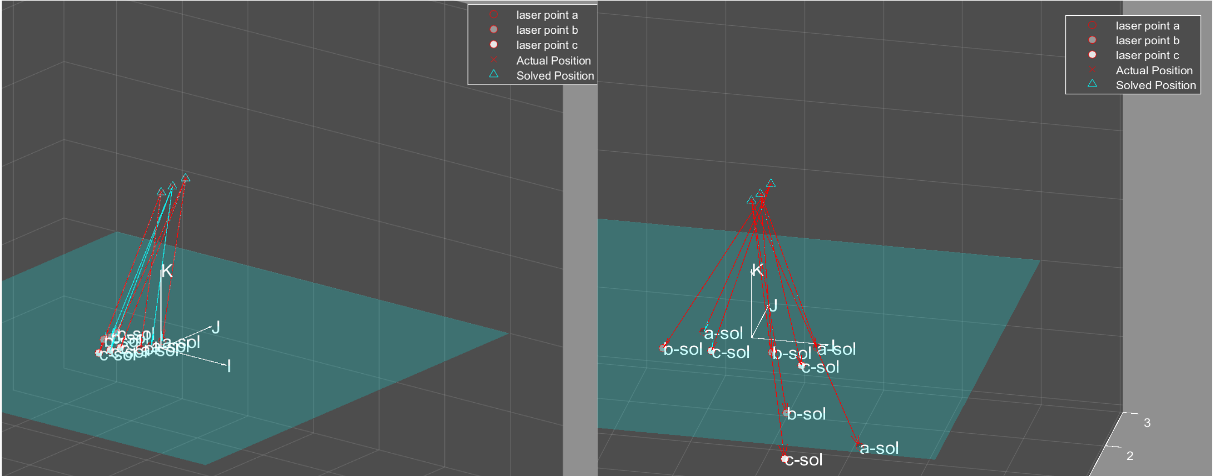
\includegraphics[width=\textwidth]{resection_fig7}
	\caption{Estimation based on prior position and new lasers endpoints small changes in orientation (Left) large changes in orientation (Right) }
	\label{fig:long2}
\end{figure*} 

After the methods passed testing in MATLAB, the program was transferred to Python showing nearly exacting results in much less time. The process operates as fast as 100Hz.

\begin{figure*}
	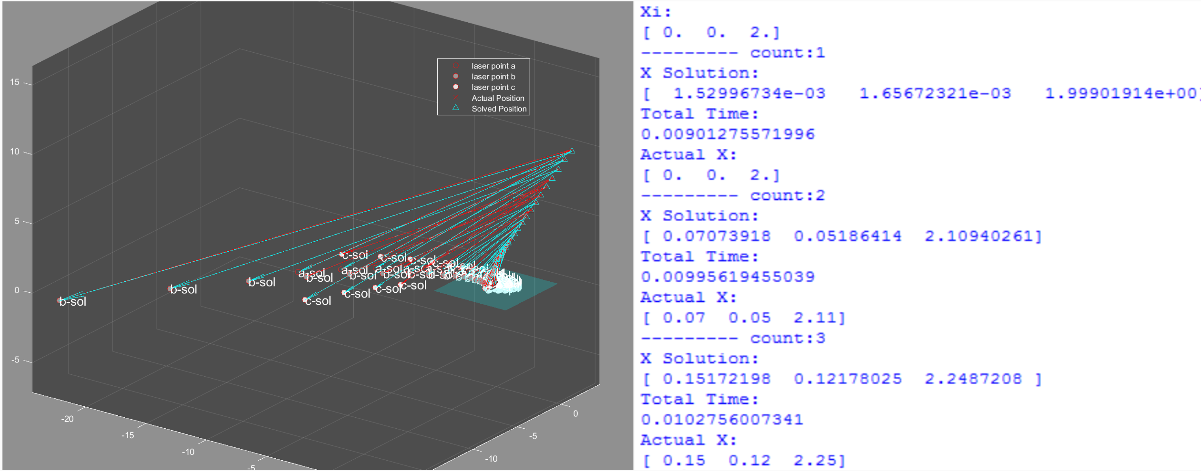
\includegraphics[width=\textwidth]{resection_fig8.png}
	\caption{Iterative simulation comparison in MATLAB and Python}
\end{figure*}

\subsection{Test Results}
The Position Estimation Program runs as one of the demos in the Laser Board Program. To begin the user selects the Laser Position Demo from the main GUI. Next the user is asked to stand at the bottom left corner of the screen at a distance equal to that of the height of the screen, wall while keeping the lasers on the board as close to the bottom left corner as possible. Once the user has done this they can press reset to initialize and run the position and orientation estimation. 
The user is given the estimated position in xyz coordinates and the orientation in yaw, pitch, and roll angles. Also the user is presented with a circle of varying location and size which is a visualization of their estimated position. 
The final results of the tracking demonstrate that position and orientation can be found with reasonable accuracy and speed. The user receives accurate position despite rotation the handles and receives accurate angle despite a change in location.  It has been found, however, that estimates can be off if the user does not take care to ensure the initialization is accurate. Also the user must ensure the in fact the lasers meet at a point. If the points do not, then the solution becomes less accurate. That is the geometry of the lasers must make a tetrahedral. 

\begin{figure}
	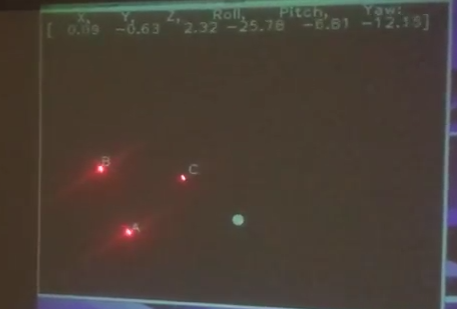
\includegraphics[width = \linewidth]{pot.png}
	\caption{A screen shot of position and orientation tracking demo \cite{techDemos}}
\end{figure}

\section{Conclusion}
We were successfully able to develop a low budget laser pointer interactive system using multiple laser pointers, a webcam and a projector. The paper went over the process required to determine the coordinate of multiple laser dots, these includes camera view homography transformation, noise attenuation, localized color intensity thresholding, and contour finding/coordinate calculation.

Using these components we were able to successfully demonstrate some simple application of our system such as basically drawing, mouse control, and maze completion games. 

The system can also be used to perform complex actions such as position and orientation tracking using 3D re-sectioning of three laser pointers.

\newpage
\eightpt
\bibliographystyle{IEEEtran}
\bibliography{final}

\newpage
\onecolumn
\section{Source Code}

Main code
\lstinputlisting[language=Octave]{LaserBoard_V7_2.py}
Laser position and orientation estimator class
\lstinputlisting[language=Octave]{LaserPosOrientEstimator.py}
	
	
\end{document}
